\chapter{Introduction, problem identification, and research goals}
\chaptermark{Introduction}

%\clearpage

\section{Introduction}

Modern technologies --- including catalysts, high-strength alloys, high-efficiency phosphors, lasers, and magnets --- are dependent upon the unique properties of the rare earth elements (REE) for their efficacy of operation.
However, global REE material-flows are prone to complex environmental, technical, and geopolitical forces on both the supply- and demand side.
Development of economically-viable technologies for the extraction of the REE and other critical materials from unconventional sources (such as geothermal fluids, oil and gas produced waters, or coal combustion residuals) has great potential value to:
generate a consistent domestic supply of materials critical to green energy and defense technologies;
valorize high-volume wastes or low-value industrial byproducts;
and avoid environmental impacts from primary REE mining.
This research seeks to address the potential for REE extraction and recovery from aqueous sources.

\section{Problem identification}

The constantly increasing consumer products incorporating the REE, and the ensuing demand for these products, have established the REE as valuable global commodities.
Domestic demand in 2012 was 11,300 tons, while the global demand was more than 113,000 tons \citep{FrostSullivan_REEmarket}.
Much of that demand is a result of a booming green energies market.
In particular, the permanent magnets sector is expected to experience significant growth between 2013 and 2020.
High-efficiency generators used in turbines and electric motors require strong and light permanent magnets.
Currently, magnets using neodymium, praseodymium, and samarium (with dysprosium and terbium additives) are the strongest and lightest commercially available.

Even at the height of domestic REE production at Mountain Pass in CA (2012), the U.S. imported \$520MM worth of REE compounds, with nearly 40\% coming from China, in order to support a demand of 11,300 tons \citep{USGS_minyb_2012}.
A booming green energies industry fueled, and continues to fuel, both domestic and global demand, where the REE provide superior performance and efficiency compared to alternative materials \citep{Nassar_JIE_2015, Graedel_PNAS_2015}.
Sustained growth in these technologies is dependent on diversifying REE sources given projected supply shortages in the medium- to long-term.
Traditional mining of REE from ore deposits is unlikely to fulfill this demand for technical and economic reasons, especially in the US where traditional mining of REE is suspended.
China, the world's leading source of REE and primary supplier of global demand for many years (Figure~\ref{fig:world-REO-prod}), has indicated partial control of exports, or punitive tariffs, in the near future.
This emphasizes the need for REE separation and recovery from unconventional matrices, such as geothermal fluids.

\begin{figure}[htbp]
\begin{center}
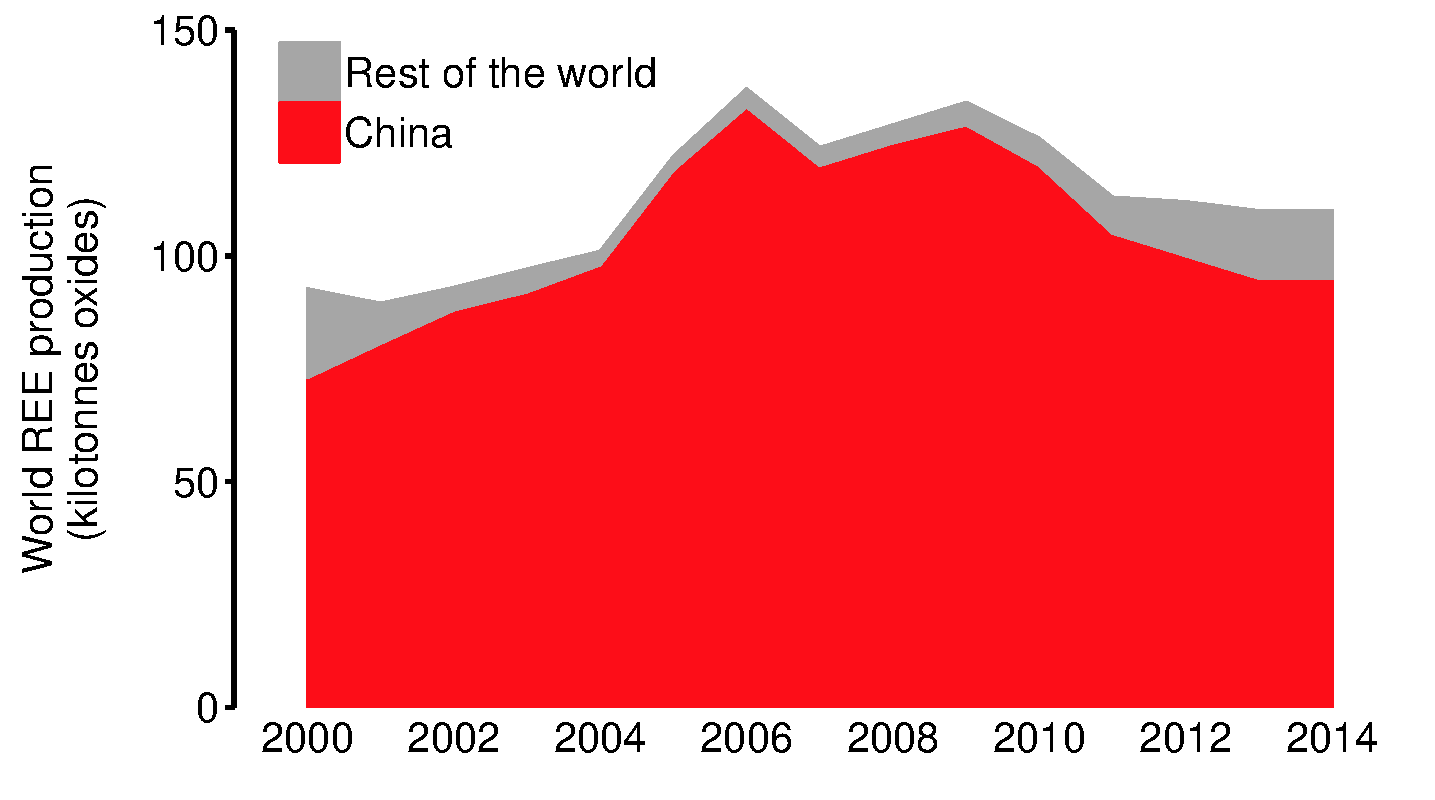
\includegraphics[width = \textwidth]{Ch1_figures/World-REO-production.pdf}
\caption[Global, primary REE production, 2000-2014.]{Global, primary REE production, 2000-2014.
Data from \citet{USGS_commsumm}.}\label{fig:world-REO-prod}
\end{center}
\end{figure}

Global REE reserves are estimated at 130 million metric tons \citep{USGS_commsumm}, much of which is located in low-concentration deposits or ocean-floor manganese nodules, which are both extremely expensive to mine with current methods.
This limits the number of readily mineable REE deposits and, ultimately, our ability to increase REE supply \citep{JRC_2011, Alonso_EST_2012}.
Aqueous media such as brines or produced waters from geothermal energy, conventional oil/gas, and shale gas extraction operations are potentially significant, but unexplored sources of REE.

Presently, REE extraction is accomplished by traditional mining (e.g. open-pit) followed by chemically-, and energy-intensive element separations, which incur a significant environmental burden (Figure~\ref{fig:Zaimes-LCA}; \citep{Zaimes_SCE_2015}).
Even when present in ores at appreciable levels, REE are commonly commingled with radioactive thorium and uranium, which need to be safely separated and stored in addition to standard waste management associated with mining (e.g. tailings) \citep{Gupta_IMR_1992, Sprecher_EST_2014}.
Stringent environmental regulations, time-intensive processes, and expensive permits complicate the opening of new, domestic mines because of these inherent risks.
On this basis, projections expect that exploiting traditional REE sources to meet increasing demand will be a significant challenge.
In 2012, China was responsible for more than 95\% of the global REE supply \citep{USGS_commsumm}.
China also had the largest demand for REE, at 66\% of the total global demand \citep{USGS_commsumm}.
The US was the next largest consumer, at 10--15\% of the total demand.
In 2011, China announced a 35\% reduction in exports of REE, in an effort to meet their domestic needs \citep{USGS_minyb_2012}.
This created large instability in the REE market as there were no other major sources for REE \citep{Alonso_EST_2012, Chakmour_Elem_2012, Hatch_Elem_2012}.
China is expected to continue reduction of exports, through either quotas or tariffs, as a mean to reduce stress on its REE reserves \citep{FrostSullivan_REEmarket, USGS_commsumm}.

\begin{figure}[htbp]
\begin{center}
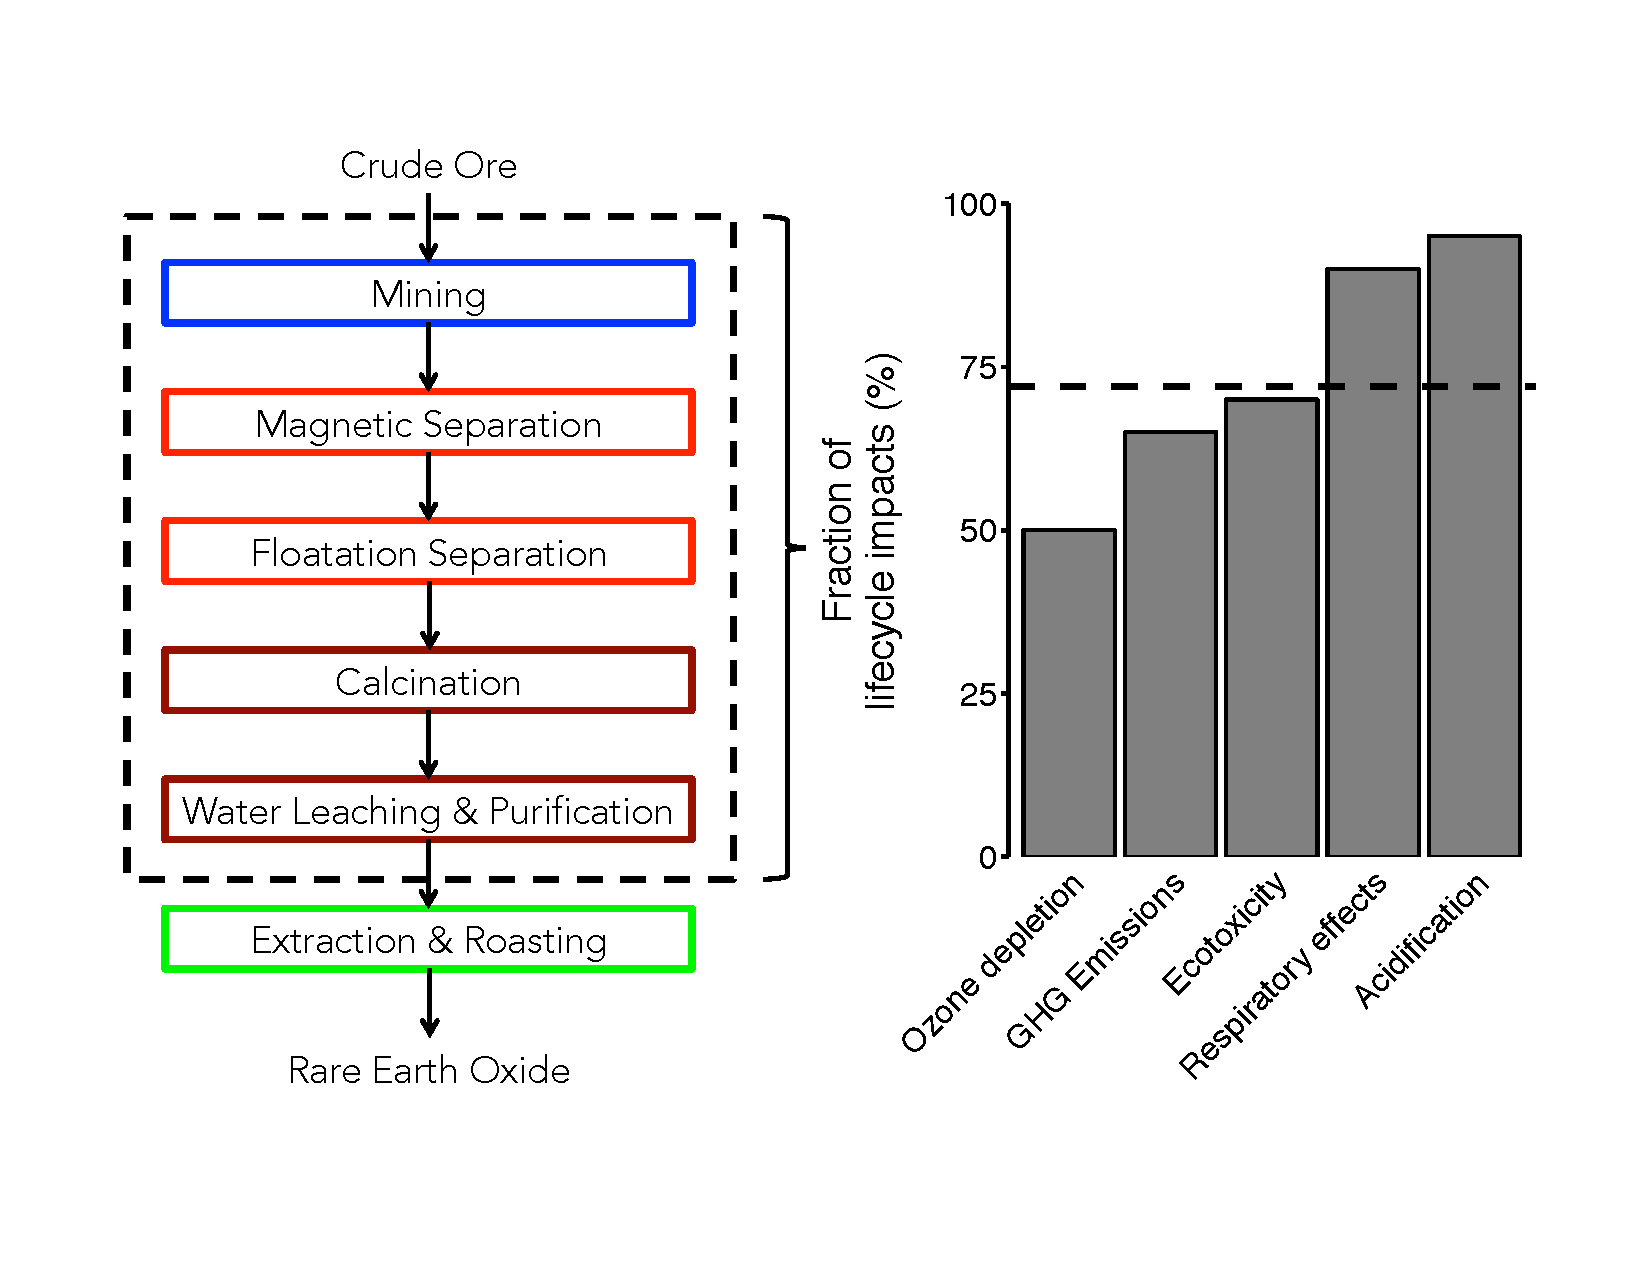
\includegraphics[width = \textwidth]{Ch1_figures/Zaimes-LCA-schematic.pdf}
\caption[Traditional REE production flowsheet (left) and the associated fraction of lifecycle environmental impacts for the boxed boundary (right) using data from \citet{Zaimes_SCE_2015}.]{Traditional REE production flowsheet (left) and the associated fraction of lifecycle environmental impacts for the boxed boundary (right) using data from \citet{Zaimes_SCE_2015}.
Only selected impact categories are shown, however the dashed line (72\%) indicates the overall average across ten categories.}\label{fig:Zaimes-LCA}
\end{center}
\end{figure}

Primary mining effectively constitutes 100\% of the REE production worldwide \citep{Binnemans_JCP_2013, USGS_commsumm},
but interest in recovery of REE from end-of-life stocks (EOL), from unconventional resources, and from REE-containing industrial wastes has expanded rapidly in recent years \citep{Binnemans_JCP_2015}.
High volumes of REE are deployed in permanent magnets, while high-value REE are used in phosphors \citep{Hatch_Elem_2012},
making these products two primary targets for recycling from EOL products along with metal hydride batteries \citep{Binnemans_JCP_2013,Tunsu_Hydro_2015}.
REE are applied in many other products, but the REE content is dissipated in-use or rendered unrecyclable by current designs \citep{Ciacci_EST_2015}.
Ferrous shredder waste (where magnets could accumulate) is a promising potential resource for REE and other critical materials.
However, \citet{Bandara_JSM_2015} propose that recycling of ferrous shredder-waste would need to exceed 50\% in order to dampen Nd price volatility from recycling alone. The conclusion from these forecasts is the need for novel, alternative feedstocks \citep{Bandara_JSM_2015}.

The United States is a pioneer in utilizing geothermal resources for the production of low-carbon energy.
Among energy production approaches, such as solar, wind, conventional oil, and coal, geothermal energy is renewable, abundant and with a small green-house gas footprint.
Although variations of geothermal power plants exist, either those being equipped with conventional hydrothermal flash-, conventional hydrothermal binary- or enhanced hydrothermal systems (Clark, Harto, Sullivan and Wang 2011),
all designs produce steam as a working fluid from naturally-heated brines found in deep, crustal reservoirs.
In a simplistic description of a steam-based geothermal power plant, high temperature brine flows to the surface from a geothermal reservoir through a production well.
This hot, pressurized fluid is separated from entrained solids and guided to gas-liquid separators, producing steam that is delivered to turbines for electricity production.
The cooled brine is mixed with condensed steam and recycled by re-injection into the reservoir without further treatment.
These fluids, where the valuable heat has already been extracted, represent an attractive source for mineral extraction that would not interfere with the primary function of the geothermal power plant.

Geothermal brines, as well as groundwater, have been reported to contain REE at typical concentrations ranging from $10^{-9}$--$10^{-12}$ g/g of solution, along with other minerals, such as Fe, Si, Al, Na, and K (Michard 1989, Lewis, Palmer, Sturchio and Kemp 1997, Lewis, Komninou, Yardley and Palmer 1998, Noack, Dzombak and Karamalidis 2014).
Depending on the reservoir lithology and the fluid chemistry (e.g. acid-sulfate, acid-sulfate-chloride, etc.), concentrations of total REE can \si{\micro}mol/kg solution ($10^{-6}$ mol/kg), as in the case of the geothermal systems from Yellowstone National Park, Wyoming, USA ,i.e. $\sum$REE = 1.13 \si{\micro}mol/kg solution, (Lewis et al. 1998).
Historical data from CDOGGR (2009) show typical geothermal brine production rates of 393,000 -- 512,000 gal/day/MWe (for a binary plant) and 93,000 -- 171,000 gal/day/MWe (for secondary flash plant).
These data optimistically translate to a maximum resource stream of 1.8 -- 2.3 mol total REE/day/MWe for a binary plant and 0.4 -- 0.8 mol total REE/day/MWe for a secondary flash plant.
Considering the total installed capacity in the US in February 2013 was 3,386 MW with new geothermal projects under development reaching 10,100 MW in 2025 (Geothermal Energy Association 2013),
creating new revenue for the industry through REE extraction from brines may be viable.
Global geothermal capacity is expected to grow from 11.6 GW in 2012 to 20.7 GW in 2020 and 29.4 GW in 2025.
The capacity expansion is largely driven by North America, Asia-Pacific as well as national and regional markets such as Turkey, Iceland and Eastern Africa (Frost  Sullivan 2014).
It is apparent that recovery of REE from these streams is a viable alternative source of critical elements both domestically and globally.

\section{Research goals}

The primary goal of this thesis research was to assess the potential for aqueous sources to serve as alternative resources for the rare earth elements.
This was accomplished through a combination of a literature analysis, analytical method development, controlled experimentation, and statistical and geochemical modeling.
Three, specific objectives were performed in order to meet this goal, with each comprising a separate chapter of this thesis.

\begin{enumerate}[label=\textbf{Objective \arabic*:}, leftmargin=*]
\item Determine the abundance of dissolved REE is waters of various compositions and investigate trends to better understand solubility controlling processes.
\item Develop an extraction and preconcentration method, robust to a range of water chemistries, for the analysis of dissolved REE in hypersaline fluids
\item Compare technologies for the economic extraction of REE from hypersaline fluids
\end{enumerate}

\subsection{REE abundance and trends in terrestrial waters}

Despite their name, the ``rare'' earth elements are ubiquitously dispersed in geologic and aqueous systems.
Study of the REE systematics in natural and anthropogenically-influenced environments has produced an extensive, but disparate, literature, holding rich insights were it to be compiled, standardized, and analyzed.
This objective brought together more than 1000 measurements from 31 studies to constitute the largest aggregation of REE data in the literature.
This objective answers question like: What is the natural variability of REE in aqueous media?
What quantitative methods exist for considering below-detection-limit values?
What is known about REE occurrence in brines?
What relationships between REE and bulk solution properties are important for REE fate and transport?
These data were used to: (1) ascertain an expected range of dissolved REE concentrations in waters of variable chemistries, deriving unbiased estimates of REE distributions and
(2) investigate trends in REE abundance in groundwater in relation to other available chemical parameters (e.g. pH, ionic strength, and major solution species).
This collection, homogenization, and analysis of a disparate literature facilitates inter-study comparison and provides insight into the wide range of variables that influence REE geochemistry.

\subsection{Analytical method development for REE measurement in hypersaline fluids}

There exists a dearth of methodologies in the analytical literature for quantitation of REE in brines by inductively coupled plasma mass spectrometry (ICP-MS).
Many approaches have been applied for separation and concentration of REE from aqueous media including solid- phase extraction (SPE), co-precipitation (co-ppt), and liquid- liquid extraction (LLE).
However, nearly all studies in the analytical chemistry literature have focused on fresh water or seawater matrices, neglecting hypersaline waters which could have significant, unknown impacts on the efficiency of separation without proper validation.

In this work, efficiency of REE separation and concentration from synthetic brines using a LLE method for quantitative analysis was studied.
The LLE method was adapted, modified, and optimized from previously published studies.
The tasks of this work were to: (1) evaluate the feasibility of REE recovery from small volumes of hypersaline solutions by LLE, (2) optimize the LLE methodology for high salinity brines, and (3) study the influence of brine composition on REE recovery.

\subsection{Novel extractive technologies for REE recovery from geothermal waters}



\section{Thesis organization}
This thesis is arranged into distinct chapters to address key knowledge- and technical gaps in the existing literature (Figure~\ref{fig:org-chart}.
The first portion deals primarily with background information to contextualize the work and identify these knowledge- and technical gaps.
Chapter 1, this introductory chapter, provides brief context to the state of the REE-economy, elucidating the benefits of developing alternative resources.
\hyperref[CH2]{Chapter~\ref*{CH2}} provides a background on the aqueous geochemistry of the REE, with a focus on complex, high-salinity systems.
The second portion constitutes the novel contributions of this thesis and is comprised of one chapter per objective (as outlined previously).
\hyperref[CH3]{Chapter~\ref*{CH3}} describes the results of a review and compilation of published REE data, accompanied by an in depth statistical analysis of occurrence distributions and trends.
\hyperref[CH4]{Chapter~\ref*{CH4}} details the optimization and application of a liquid-liquid extraction to precisely measure REE concentrations in small volumes of complex, hypersaline fluids.
\hyperref[CH5]{Chapter~\ref*{CH5}} characterizes the performance of surface attached ligands for the extraction and recovery of the REE from synthetic brine solutions.
Finally, \hyperref[CH6]{Chapter~\ref*{CH6}} summarizes this project in the broader context of alternative REE resources and suggests future work.

\begin{sidewaysfigure}[htbp]
\centering
\begin{forest}
    for tree={
      if level=0{align=center}{
      		if level=1{ align={@{}C{75mm}@{}} }{ align={@{}C{25mm}@{}} }
	},
	if level=3{ align={@{}C{75mm}@{}} }{}, 
%      draw,
%      edge path={
%        \noexpand\path [draw, \forestoption{edge}] (!u.parent anchor) -- +(0,-5mm) -| (.child anchor)\forestoption{edge label};
%      },
      parent anchor=south,
      child anchor=north,
      l sep=10mm,
      tier/.wrap pgfmath arg={tier #1}{level()}
    }
    [\textbf{Measurement and Recovery of Rare Earth Elements from Hypersaline Fluids}
      [Background material
      	[{Introduction, problem identification, and research goals}]
	[Aqueous chemistry of the rare earth elements (REE)]
	[Review of current and proposed REE extraction techniques] 
      ]
      [Novel contributions
        [\textit{Objective 1:}\\Determine REE abundance and trends in terrestrial waters, name = O1]
        [\textit{Objective 2:}\\Develop efficient extraction technique for measurement of REE in hypersaline fluids
        		[Broader impacts and future work, name = BIFW]
        ]
        [\textit{Objective 3:}\\Compare technologies for the economic extraction of REE from hypersaline fluids, name = O3]
      ]
    ]
    \draw (O1.south) -- (BIFW.north);
    \draw (O3.south) -- (BIFW.north);
  \end{forest}
\caption{Organization of the thesis, including research objectives}\label{fig:org-chart}
\end{sidewaysfigure}

%\tikzstyle{io} = [trapezium,
% trapezium left angle=70,
% trapezium right angle=110,
%% minimum width=3cm,
%% minimum height=1cm,
% text centered,
% draw=black,
% fill=blue!30
% ]
% 
% Here is some test with my drawing \protect\tikz\protect\node[draw, io]{trapezoid}; in between text.


\bibliographystyle{unsrtnat}
\bibliography{Ch1_bib}